\subsection{Code Generator}

In this section you will learn how to implement the code generator for 
the target application. For simplicity, the code generator templates are placed
in the \texttt{org.eclipse.xtext.example.ql} project in a sub-package \texttt{generator}. 
Usually it would be better to create a separate project which contains the generator,
since the language is independent from a single target platform. It would
be possible to create different code generators for different target platforms,
and it would be better to implement each of them as separate projects.

Generator templates in Xtend are implementations of the \texttt{IGenerator}
interface:

\begin{lstlisting}[language=Java]
package org.eclipse.xtext.generator;

public interface IGenerator {
	/**
	 * @param input - the input for which to generate resources
	 * @param fsa - file system access to be used to generate files
	 */
	public void doGenerate(Resource input, IFileSystemAccess fsa);
}
\end{lstlisting}

\subsubsection {Dispatcher template}

The code generator is invoked with a \texttt{Resource} instance, which holds a \texttt{Questionnaire}
instance. We have to generate multiple artifacts for each resource, so it is a common 
pattern to create a template class which serves as entry point and dispatches to other
template classes to create the artifacts. Usually one template per artifact is
created.

Create the class \texttt{Root.java} in package \texttt{org.eclipse.xtext.example.ql.generator}:

\begin{lstlisting}[language=Java]
package org.eclipse.xtext.example.ql.generator;

import javax.inject.Inject;

import org.eclipse.emf.ecore.resource.Resource;
import org.eclipse.xtext.generator.IFileSystemAccess;
import org.eclipse.xtext.generator.IGenerator;
import org.eclipse.xtext.xbase.compiler.JvmModelGenerator;

@SuppressWarnings("restriction")
public class Root implements IGenerator {
  @Inject
  JvmModelGenerator jvmModelGenerator;

  public void doGenerate(Resource input, IFileSystemAccess fsa) {
    // dispatch to other generators
    jvmModelGenerator.doGenerate(input, fsa);
  }
}
\end{lstlisting}

As a first generator to which is dispatched, we inject an instance of
\texttt{JvmModelGenerator}. This is a standard generator shipped with Xtext which
translates types inferred by the Jvm Model Inferrer to Java classes.
In our case, the Java class for Forms are generated by the
\texttt{JvmModelGenerator}. In JSF terms, we speek of the \emph{Backing Bean}.
 
Next, Xtext has to know that \texttt{Root} is the template that has to be invoked
as generator implementation. This has to be configured - you guessed right! - 
with Guice again. We need to add a configuration that binds the \texttt{IGenerator}
interface to the \texttt{Root} class.

Open class \texttt{QlDslRuntimeModule} and add this method:

\begin{lstlisting}[language=Java]
  @Override
  public Class<? extends IGenerator> bindIGenerator() {
    return Root.class;
  }
\end{lstlisting}

Now we are ready to add additional templates and register them in the
\texttt{Root} class.

\subsubsection {JSF Generator}

For that purpose we use the \texttt{New Xtend Class Wizard} to create a
new Xtend file \texttt{JSFGenerator.xtend} in package
\texttt{org.eclipse.xtext.example.ql.generator}.

\begin{center}
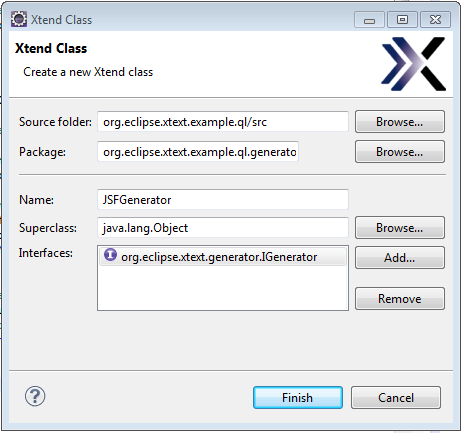
\includegraphics[width=10cm]{./images/chapter02/newXtendClassWizard.png}
\end{center}

The \texttt{New Xtend Class Wizard} provides the possibility to add interfaces
by use of the \texttt{Add} button near the interface section. As we want to
create a new generator we add the interface
\texttt{org.eclipse.xtext.generator.IGenerator} to our new Xtend class.

\begin{center}
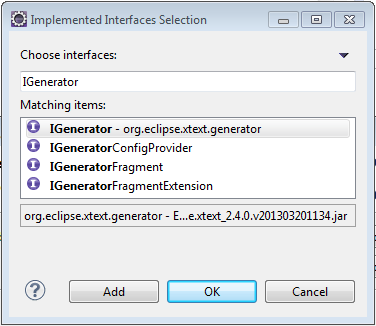
\includegraphics[width=10cm]{./images/chapter02/newXtendClassWizardAddInterface.png}
\end{center}



- create xtend file
- add xtend lib if required
- show whole generater
- explain step by step

